\label{sec:classification}
Nachdem in vorherigen Abschnitt eine passende Merkmalsmenge erstellt wurde, geht es nun um die Entscheidung, ob der Fahrer Müde oder Wach ist bzw. ob das System eine Müdigkeitsmeldung erscheinen lässt. Für diese Klassifizierung werden im allgemeinen Machine-Learning-Algorithmen verwendet. Anhand von markierten Datensätzen wird versucht den Algorithmus zu Trainieren (Überwachtes Lernen). Dies dient dem Ziel, dass er auch unbekannte Daten klassifizieren kann. Dieser Vorgang wird Generalisierung bezeichnet und ist auch im menschlichen Lernen ein wichtiger Schritt.

Für die Anwendung wurde zur Klassifizierung ein künstliches Neuronales Netz (KNN) ausgewählt. Es basiert auf einem erweiterten Perceptron / McCulloch-Pitts-Neuron \cite{ann} und ist der Funktionsweise des menschlichen Gehirns bzw. seinen Neuronen nachempfunden\cite{marsland_opac-b1129336}. Ein KNN lässt sich im einfachste Fall durch eine Merkmalsmenge $X = x_1, x_2 ... x_n$, dazugehörige Gewichte $W = w_1, w_2 ... w_n$, eine Übertragungsfunktion $\sum$ und eine Schwellwertfunktion $\theta$ beschreiben (Abb. \ref{fig:perceptron}).

\begin{figure}[h] 
  \begin{center}
    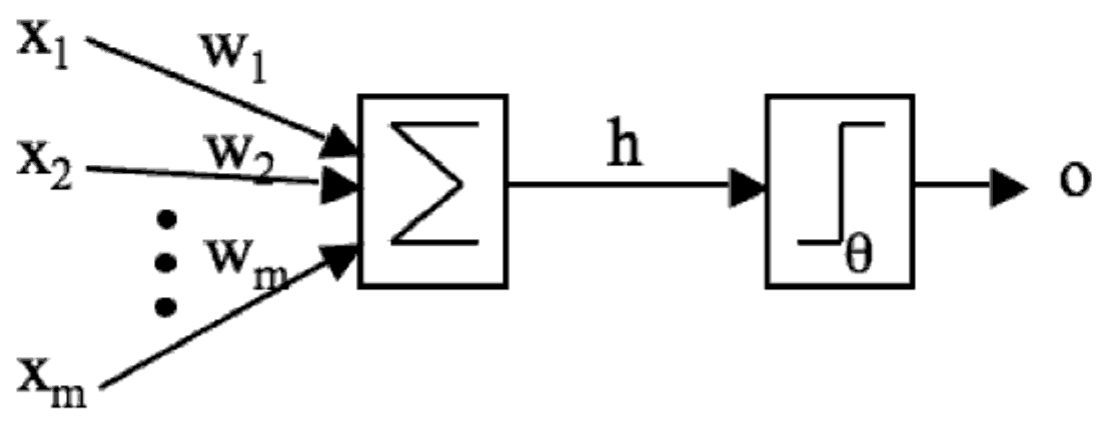
\includegraphics[width=5.5cm]{perceptron}
    \caption[Schema eines Perceptrons / McCulloch-Pitts-Neurons]{Darstellung eines McCulloch-Pitts-Neurons. Die Merkmale $X$ werden mit den Gewichten $W$ multiplziert und in $\sum$ summiert. Wenn $h > \theta$ "`feuert"' das Neuron ($o = 1$) \cite{marsland_opac-b1129336}. \label{fig:perceptron}}
  \end{center}
\end{figure}

Dieser Aufbau kann schon einfach Aufgaben, wie bspw. ein logisches "`UND"', lösen. Jedoch lässt sich schon ein logisches "`XOR"' nicht mehr abbilden. Dafür müssen weitere Schichten von Neuronen (Hidden Layers) hintereinander geschaltet werden - das sog. Multi Layer Perceptron (MPL, Abb. \ref{fig:mlp}).

\begin{figure}[h] 
  \begin{center}
    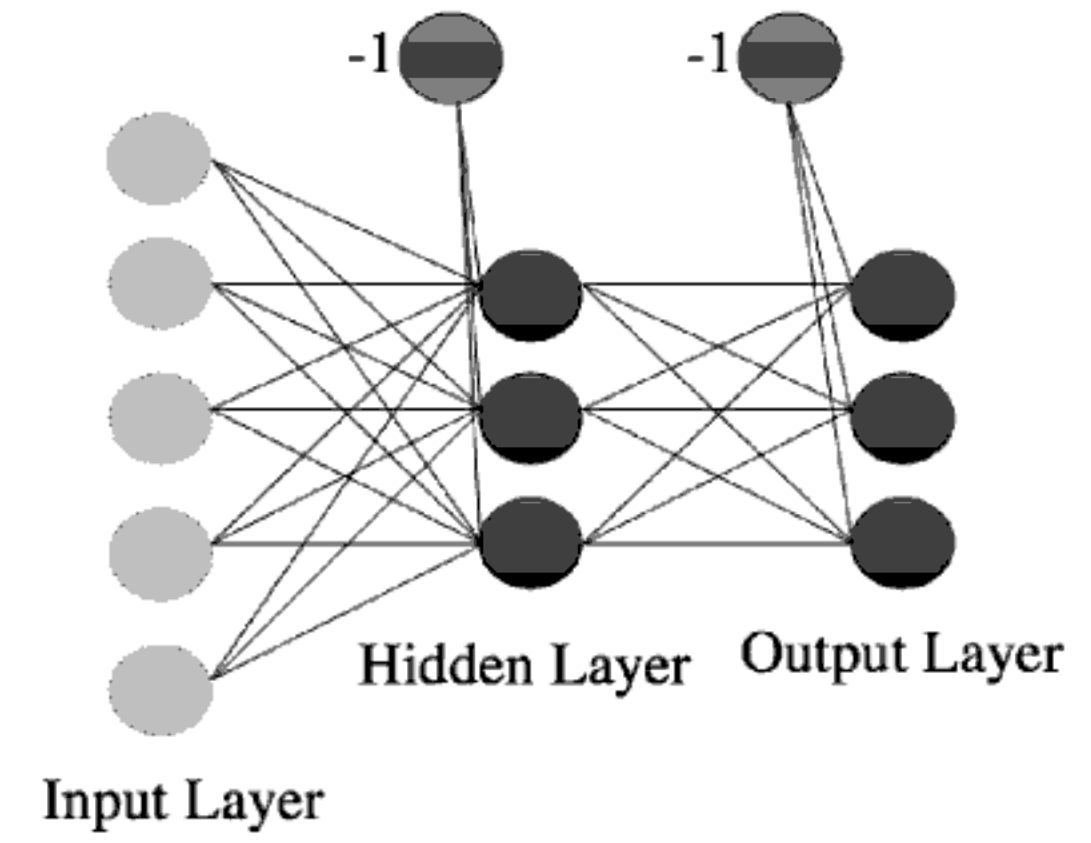
\includegraphics[width=5.5cm]{mlp}
    \caption[Schema eines Multi-Layer-Perceptrons]{Darstellung eines Neuronalen Netzes mit mehreren Schichten (Multi Layer Perceptron, MLP)\cite{marsland_opac-b1129336}. \label{fig:mlp}}
  \end{center}
\end{figure}

Es exisitiert kein bekannter Algorithmus für die Wahl der optimalen initialen Parameter eines KNNs. Vuckovic et al. \cite{Vuckovic2002349} hatten sich mit diesem Thema genauer beschäftigt und die Ergebnisse werden für die Versuche herangezogen.

Die Merkmalsvektoren kommen zu gleichen Teilen aus der Wach und Müde-Menge und sind mit den jeweiligen Klassen 0 und 1 versehen. Insgesamt wurden 1170 Datensätze mit jeweils 24 Werten pro Vektor eingesetzt. Vor dem Training wurde die Merkmalsmenge in Trainings- und Testmenge (2:1) aufgeteilt. Intern wird beim Training noch einmal ein Teil der Daten zum validieren genutzt (15\%). So wird sicher gestellt, dass die Tests nie mit Daten durchgeführt werden, die schon beim Training genutzt wurden. Sonst kann es zum sog. Overfitting kommen, das bedeutet, dass das Netz zu genau auf die Trainingsdaten eingestellt ist und nicht mehr generalisiert.

Für die Anwendung wurde das Training des KNN mit verschiedenen Parametern durchgeführt. Die Menge der Eingabevektoren (X) ist durch die Größe des Merkmalsvektors vorgegeben. Da lediglich 2 Klassen (Wach und Müde) existieren, reicht ein binärer Ausgabevektor aus. Die Frage nach der Menge der Hidden Layer lässt sich nicht per se beantworten. In Versuchen ergaben 2 und 4 Schichten die besten Ergebnisse. Weitere Parameter können beim Training eingestellt werden, ein variabler Trägheitsterm (Momentum) verhindert bspw. das Feststecken in lokalen Minima, die Lernrate steuert die Lerngeschwindigkeit im Vergleich zu Genauigkeit. Gute Ergebnisse ließen sich mit einem Momentum 0,1 und einer Lernrate von 0.005 erzielen.

Die Testmenge wird nun in das KNN eingegeben und überprüft, ob der richtige Klasse erkannt wird. Daraus ergibt sich eine Ergebnis-Matrix \ref{tab:ann_results}, in der jede richtig und falsch erkannte Klassifizierung ersichtlich wird. Die Diagonale zeigt die richtig erkannten Klassen und in der letzten Spalte lässt sich die Erkennungsrate pro Klasse erkennen. Da beide Klasse zu gleichen Teilen vorhanden sind, ist die  Gesamt-Erkennungsrate das Mittel der beiden Einzelraten.

\begin{table}[t]
 \centering
 \caption{KNN Ergebnis-Matrix}
 \begin{tabular}{l|lll}
   & Wach & Müde & Erkannt \\ \hline
  Wach & 75 & 25 & 75\%\\  
  Müde & 75 & 75 & 25\%\\ 
  Gesamt & - & - & 50\%\\ 
 \end{tabular}
 \label{tab:ann_results}
\end{table}